\chapter{Results interpretation}

Based on the results of the different experiments I made, I will try to answer in this chapter to three main questions:
\begin{enumerate}
  \item Compared to other available solutions, how good is the current configuration chosen by INGInious to face the responsiveness challenge of the platform?  How much better could it be?  How easy would it be to improve it?  Do some solutions involve trade-offs in terms of maturity, support or maintainability?
  \item Could there be a solution tailor-made for the specific case of INGInious?  What would it be?  What would it cost to use it?
  \item What would be the cost of providing stronger/safer isolation to the containers used by INGInious?  Which opportunities could it bring?
\end{enumerate}

\section{Current INGInious situation}
We will here consider the first question:
\begin{center}
  \say{\textit{Compared to other available solutions, how good is the current configuration chosen by INGInious to face the responsiveness challenge of the platform?  How much better could it be?  How easy would it be to improve it?}}
\end{center}

The current configuration of INGInious is the following:
\begin{center}
\begin{tabular}{rl}
  \textbf{Container manager} & Docker \\
  \textbf{Base image} & Centos \\
  \textbf{Storage driver} & overlay2 \\
  \textbf{Container runtime} & runc \\
  \textbf{Control group version} & v1 \\
  \textbf{Rootless containers} & no \\
\end{tabular}
\end{center}

This configuration is quite decent and gives good performances, there is mainly one change that can improve those.  But let's analyze this step by step.

\subsubsection{Storage driver}
Overlay2 (referenced for the rest of this discussion as simply overlay) is the storage driver that Docker recommends to use by default (when OverlayFS is supported on the host).  Its layer mechanism allows you to limit the redundancy of information when you use the same base image to create different images.  And its file-based copy-on-write strategy gives overall good performances.

\begin{figure}[h!]
  \begin{center}
    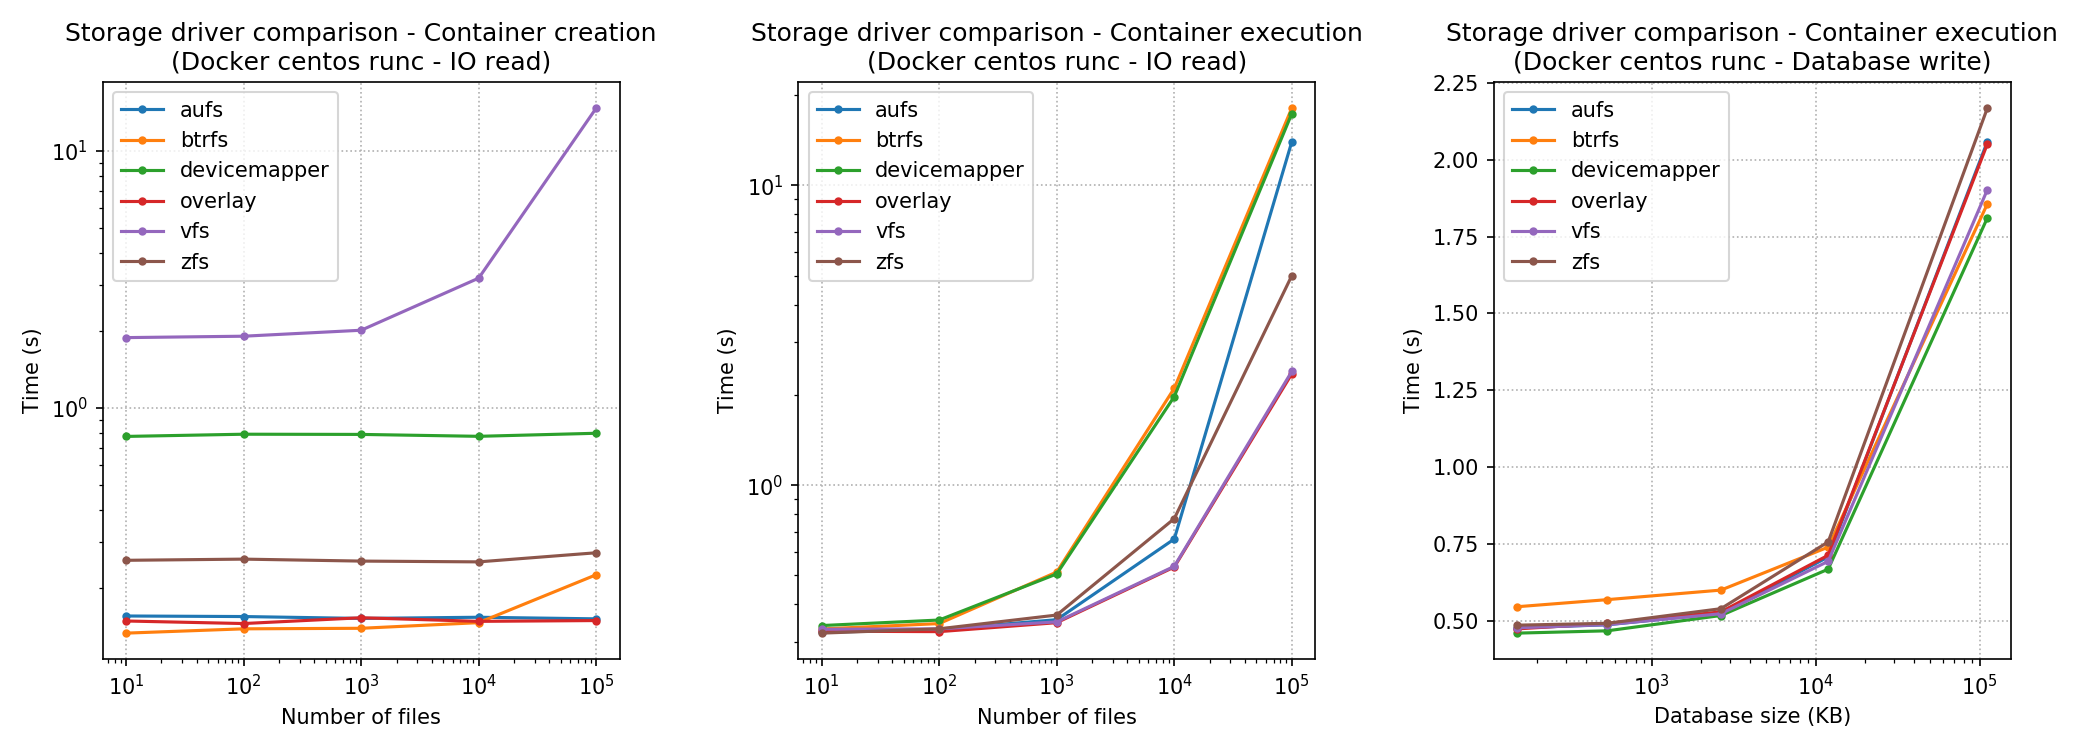
\includegraphics[width=\linewidth]{images/question-1-storage-driver.png}
    \caption{Storage driver performance comparison for Centos containers, launched with Docker and runc}
    \label{fig:q1:storage-driver}
  \end{center}
\end{figure}

In Figure \ref{fig:q1:storage-driver}, we can see how much it cost to have a full-copy mechanism like vfs for each container creation.  We can also see that overlay, aufs and btrfs offer similar performances for the creation of containers.  The main differences between those three are shown by their performance when soliciting I/O.  
\begin{itemize}
  \item Aufs, even though performing similarly to overlay in all the other cases (not shown here) and relying on the same union file system mechanism as overlay, gets far behind the latest when a lot of reading operations are done.  This most likely comes from one big difference in the implementation of those two union file system: when a file is opened with OverlayFS, all the operations on it are directly managed by the underlying file systems.  This simplifies the implementation and improves the performances quite a lot as we can see in the second graph of the figure.  (For this test, for each \texttt{openat} system call, four \texttt{read} system calls are done)
  \item On the last graph of the figure (on the right), we can see the advantage of using block-based copy-on-write, when modifying big files.  Indeed, when doing so, where overlay and aufs will need to copy the whole file before modifying it, the other solutions will only need to copy the file system blocks needing to be modified (or not even copy the file in the case of vfs).  We can see that devicemapper handles this a little bit better than btrfs, but given the much higher container creation cost of the first one, it will most likely be more interesting to use btrfs in most cases.
  \item One more thing to pay attention to is that storage drivers with block-based copy-on-write mechanisms seem to face some difficulties when creating containers with a large number of files in it.  This might be harder to see here for devicemapper and zfs, but it is the case.  Zfs seems to also suffer from big files in the container filesystem when creating containers.
\end{itemize}
One more reason to justify the use of overlay is that in most container use cases, read operations are the most important ones.  Normally, no large amount of data should be written in the container file systems, volumes (external storage from the host, mounted into the container file system) should specifically be used for that purpose as it provides nearly native writing performances and the data persists, even after the end of the container life cycle.

In terms of maintainability, one thing to pay attention to is that Docker sometimes stops the support for some storage drivers.  It already occurred for devicemapper since version 19.03, and might be the case soon for aufs too.

\subsubsection{Base image}

Alpine is quite popular in container file systems.  Thanks to its minimalist default configuration, its image is quite light compared to the ones of more complete file systems.  The Alpine base image provided by Docker is only $5.61$\texttt{MB}, while Centos's one is $203$\texttt{MB}.  But the size taken by images on disk is not something we worry about in our case as it will not have any impact on the user experience.

\begin{figure}[h!]
  \begin{center}
    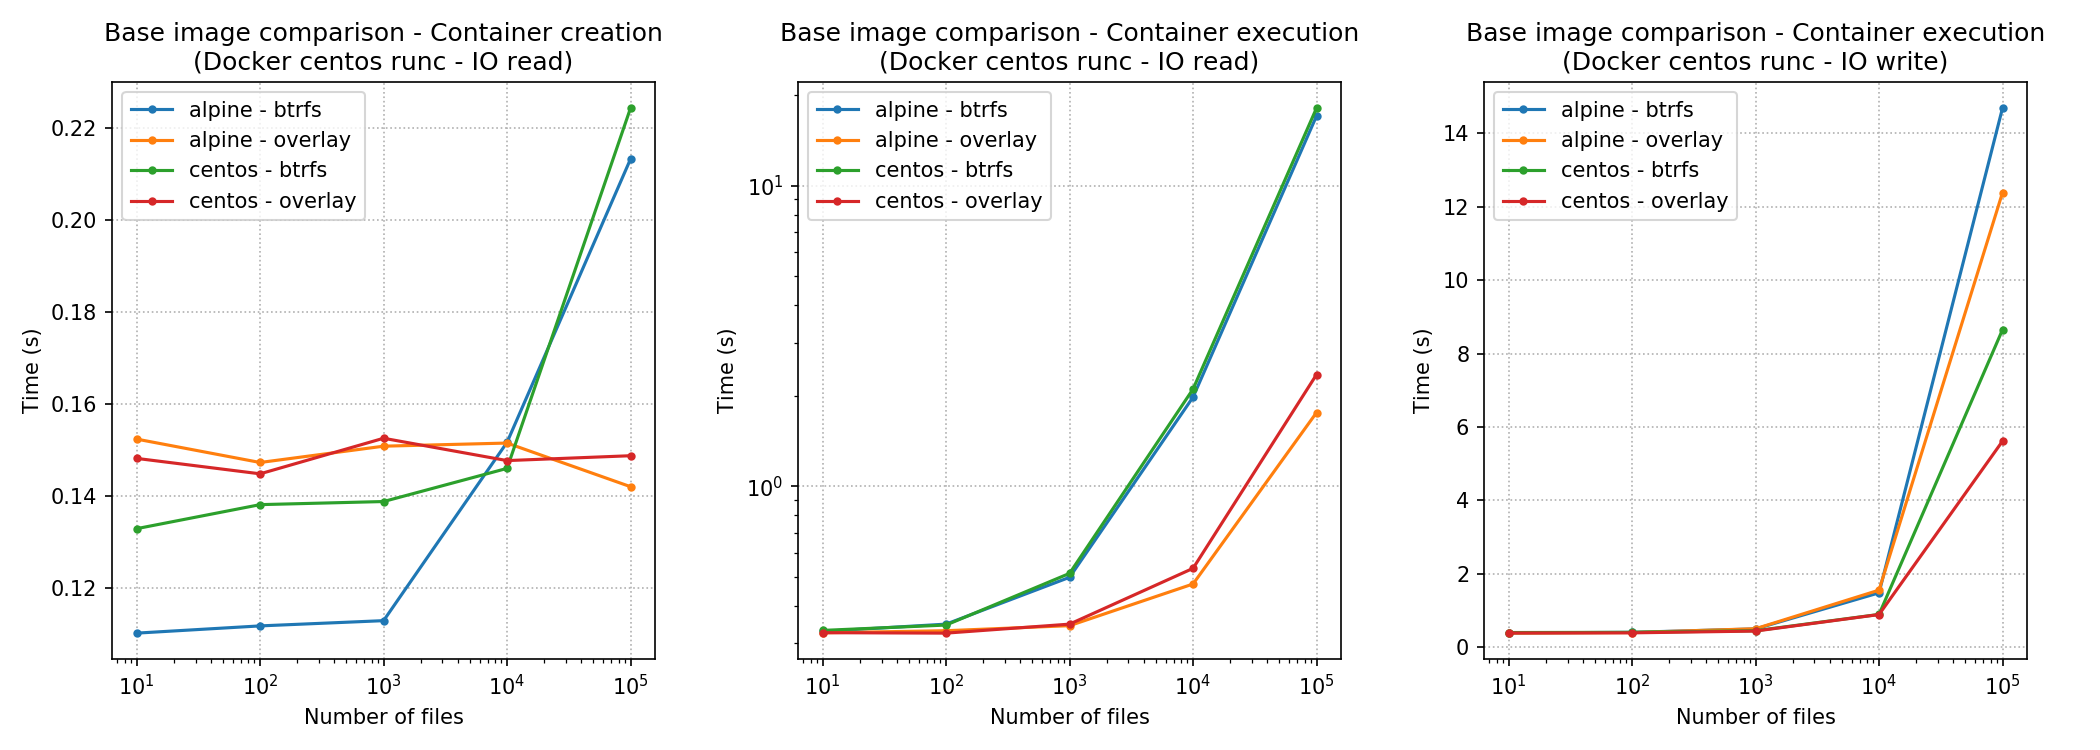
\includegraphics[width=\linewidth]{images/question-1-base-image.png}
    \caption{Base image performance comparison for containers launched with Docker and runc}
    \label{fig:q1:base-image}
  \end{center}
\end{figure}

From the graphs of Figure \ref{fig:q1:base-image}, we can notice several things:
\begin{itemize}
  \item We can see on the first graph (on the left) that, once more, btrfs offers better creation performances when the number of files is smaller.  Therefore, Centos being a more complete Linux distribution than Alpine, with more functionalities, and so, more files, the creation performance with this storage driver will be poorer than when Alpine.
  \item On the second graph, it also appears that simple read operations are a little bit faster when using Alpine as a base image.  This trend has also been observed with big file reading, with the \textit{Database read} test.
  \item One thing really interesting that we can see on the last graph, however, is that the trend seems to be inverted for write operations.  This difference is likely to be caused by the difference in the implementation of \texttt{tar} (used for this test) in each distribution's package repository.  Indeed, the implementation coming from Alpine makes a lot more system calls (about three times more) than Centos's one.
\end{itemize}

The choice of Centos as a base image can then be justified by the maturity of such distribution.  It had been around for a while, it is widely used outside of container applications, and is more likely to count optimization in the different tools at disposal.  When those tools are not required though, the minimalist design and lightweightness of Alpine make it a better choice.

\subsubsection{Container runtime}

On Figure \ref{fig:q1:runtime} is shown the influence of different container runtime solutions on the different execution steps of the container.  

\begin{figure}[h!]
  \begin{center}
    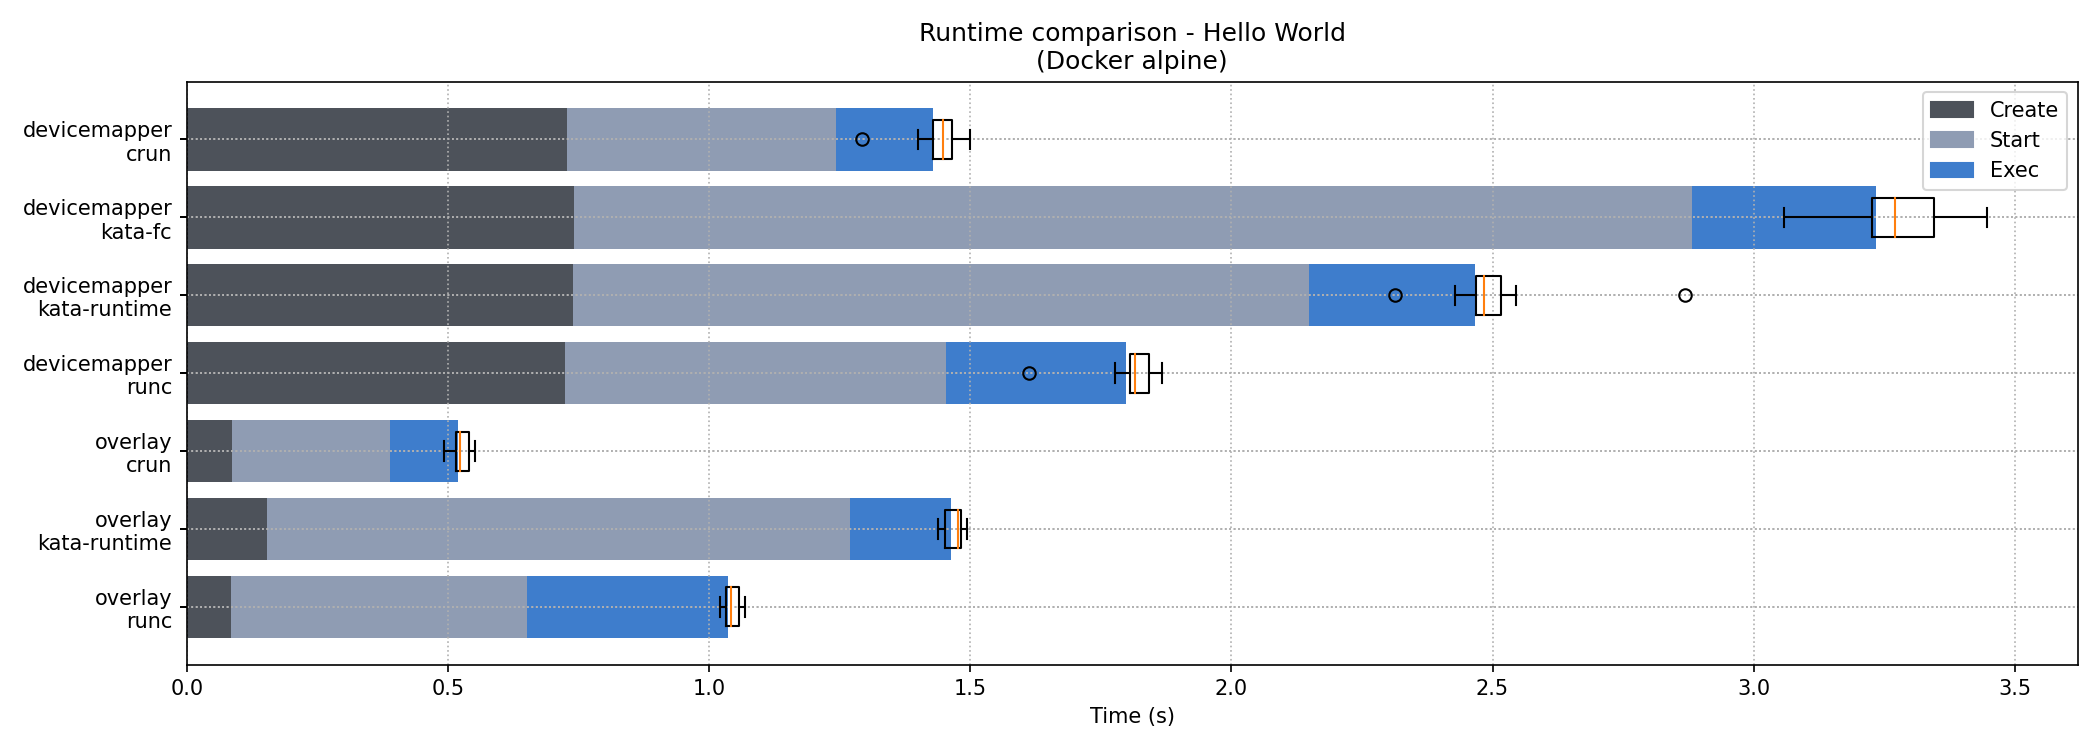
\includegraphics[width=\linewidth]{images/question-1-runtime.png}
    \caption{Runtime performance comparison for Alpine containers, launched with Docker}
    \label{fig:q1:runtime}
  \end{center}
\end{figure}

By first comparing crun to runc, we see how much of a difference it makes to use an efficient C implementation, over a less efficient Go one.  The difference is much more obvious for the \texttt{start} and \texttt{exec} phases as those are the steps where real low-level operations are made by the container runtime (entering namespaces, setting cgroups, forking processes).  

Then we have the Kata Containers solutions, based on virtualization.  It obviously will lead to a greater overhead for creating and starting containers, as a whole kernel has to be loaded.  However, the \texttt{exec} phase seems to have much lower overhead.  We can not miss how much worse is \texttt{kata-fc} (using Firecracker hypervisor) compared to \texttt{kata-runtime}, and it might be disappointing given the recent popularity that has embraced Firecracker.  In response to that here are some important elements:
\begin{enumerate}
  \item Firecracker has not been conceived to run under Kata Containers' hood.  It might perform better when running standalone.
  \item Some advantages that Firecracker has and which are not obvious in our study case are, firstly, the memory footprint, which is way smaller than with Qemu, and secondly, the reduced code base, which ensures a much lower attack surface.  Those are also reasons why Firecracker is so popular.
  \item After some discussion with Kata Containers community\footnote{The full discussion can be found at this link: \href{https://github.com/kata-containers/runtime/issues/2642}{https://github.com/kata-containers/runtime/issues/2642}}, it turned out that Kata Containers make use of one feature of Qemu that Firecracker does not have, that would justify this difference in performance: vNVDIMM.  Thanks to vNVDIMM, the root file system of the guest VM is fully loaded in memory and directly accessed in it, which is faster than reading it from disk as Firecracker does.
\end{enumerate}

All those runtimes are completely mature alternatives, with great support, a community behind it and a large user base.  

\subsubsection{Container manager}

On Figure \ref{fig:q1:manager} are shown the different container manager considered in the experiments, in the configuration that my tests revealed as most performant.  Docker and Podman using crun as runtime, and overlay or btrfs as storage driver.  LXD uses LXC as runtime and btrfs as a storage driver.

\begin{figure}[h!]
  \begin{center}
    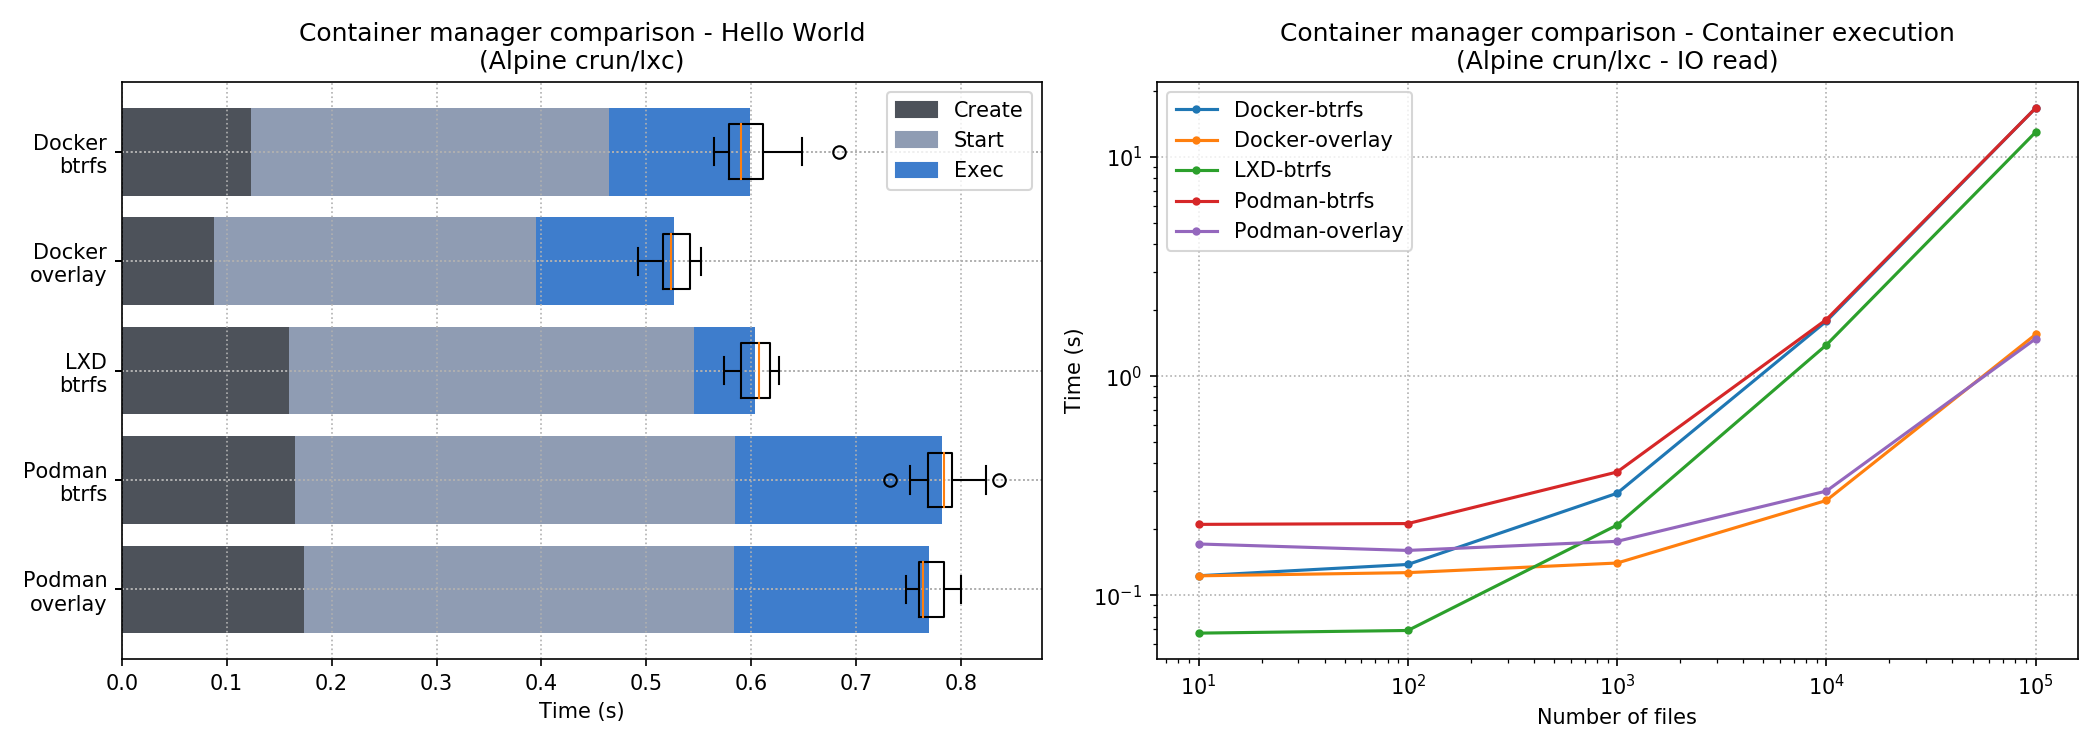
\includegraphics[width=\linewidth]{images/question-1-manager.png}
    \caption{Container manager performance comparison for Alpine containers}
    \label{fig:q1:manager}
  \end{center}
\end{figure}

We can see that Docker is still the best solution for us, even though none of the other solutions presents really bad performances.  Given the relatively young age of Podman, its focus might not be yet fully on performances, but rather on functionalities, catching up all the things that the two other alternatives already have.  We can then hope for improvements on this as time goes.  It would be worth check on them later this year, or the next one.  

All those three solutions are reliable, have great support, and a community to back them up.  LXD is maintained by canonical, which makes it a great fit for Ubuntu environments.  Docker is maintained by Docker Inc. and also seems to bring greater support for Ubuntu.  Podman is supported by the containers\footnote{\href{https://github.com/containers}{https://github.com/containers}} organization and is served as default Docker alternative on Fedora.  Using Podman on Ubuntu has been a bit more complicated than the two others, especially for the rootless solution, which requires cgroupv2.  Thankfully the community offered great support for all of my problems, and in most cases, the issues appeared to be with systemd or Ubuntu, rather than with Podman\footnote{The full discussion for the issue I had can be found here: \href{https://github.com/containers/libpod/issues/6368}{https://github.com/containers/libpod/issues/6368}}.

One last positive point to give to Docker is also its documentation.  Even though there is also documentation for the other tools, it is much more complete on Docker's side.  And Docker being also the most popular solution, a lot of complementary information, blog posts, stack overflow threads, are available online too.

\subsubsection{Final configuration}

Based on the previous observations, the ideal configuration would then be:

\begin{center}
\begin{tabular}{rl}
  \textbf{Container manager} & Docker \\
  \textbf{Base image} & Alpine/Centos \\
  \textbf{Storage driver} & overlay2 \\
  \textbf{Container runtime} & crun \\
  \textbf{Control group version} & v1 \\
  \textbf{Rootless containers} & no \\
\end{tabular}
\end{center}

As we can see, the final configuration is not that much different from the original one.  
\paragraph{}The quick answer to the original questions "\textit{Compared to other available solutions, how good is the current configuration chosen by INGInious to face the responsiveness challenge of the platform?}" would be:
The current configuration is good.  It could be improved but it is not the worst one.  The choice of going with Docker was the obvious choice when INGInious was created, and it is still the case now.  The current storage driver offers great performances for almost every case, only some specific case, soliciting a lot of IO operations on big files, can give an advantage to another storage driver, btrfs.  The choice of a Centos base image is not bad either, but the size of the image being greater than Alpine's one makes it less ideal for containerization applications.  Except for the situations where Centos offered better write performances, using Alpine seems to be better.  The move here might then be to go for a hybrid solution, using Centos only in situations where its small writing performance advantage becomes meaningful.  
\paragraph{}\textit{How much better could it be?}  As we have seen, changing the current container runtime makes a significant difference.  The c implementation of \texttt{crun} is claimed to be twice as fast as the go implementation of \texttt{runc} by \texttt{crun}'s contributors.  And we can see the difference.  The change of base Image though does not show an obvious improvement.
\paragraph{}\textit{How easy would it be to improve it?}  This is the real good news, it truly is super easy to apply the most significant change.  You only need to install \texttt{crun}, reconfigure Docker to use it by default, and we are good to go, no change as to be done to INGInious!  For the choice of the base image though, the story is different, as it would require to change all the containers images, which is a lot of work.
\paragraph{}\textit{Do some solutions involve trade-offs in terms of maturity, support or maintainability?}  All of the solutions I explored here are reasonable to use, none of them have weak support or lack of maintainability or stability.  But as discussed, some storage driver might lose their support on Docker's side and Docker is better documented than the other container manager.

\paragraph{}\textbf{Note about Http Serveur and Ping test}:  The results of the different configuration to those tests were not presented here and will not be shown later.  This is because no additional information could be extracted from those.  The performances to Http Server test are in pairs for each configuration with its result to the Hello World test.  Regarding the Ping test, the variations were too small to assume a difference in performance rather than the varying network load.  If this test has to be reproduced, it might be interesting to ping a target in a private network that we have under control, rather than the internet. More graphs can be found on the repository of this project at this address: \href{https://github.com/edvgui/LEPL2990-Benchmark-tool/tree/master/plots}{https://github.com/edvgui/LEPL2990-Benchmark-tool/tree/master/plots}.

\section{INGInious ideal solution}
We will here consider the second question:
\begin{center}
  \say{\textit{Could there be a solution tailor-made for the specific case of INGInious?  What would it be?  What would it cost to use it?}}
\end{center}

The different container managers presented here are very versatile solutions, they all have a great package of functionalities that allows them to deal with a wide range of different applications.  This is good for them, but bad for us, as we do not need most of those functionalities, but still pay the cost through a heavier container manager.

The workload that INGInious handles with its container manager is not that extensive, it is even quite redundant, and predictable, as each student's code is expected to have a specific behavior.  And that expected behavior can define, in advance, which files in the container filesystem are going to be modified, and which are not.  We can play with that knowledge.

I have then created a concept alternative solution, Contingious, that would just fit the needs of INGInious, and provide better performances.  It relies on two things:
\begin{enumerate}
  \item We do not need a fully functional and grown-up container manager. Our needs are simply containers, with resource management.  Those are provided by tools like crun and runc and cgroup v1 and v2.  We could then gain performance by only using those.
  \item We do not need a complete writable filesystem for each container, we can restrict write access to certain parts of it.  This means that we could copy the file that will be modified when creating the container (avoiding the need of using any copy-on-write mechanism), and bind-mount the rest of it, with read-only permissions.
\end{enumerate}

The full current implementation and some more implementation details can be found in the repository of this project at this address: \href{https://github.com/edvgui/LEPL2990-Benchmark-tool}{https://github.com/edvgui/LEPL2990-Benchmark-tool}.

\begin{figure}[h!]
  \begin{center}
    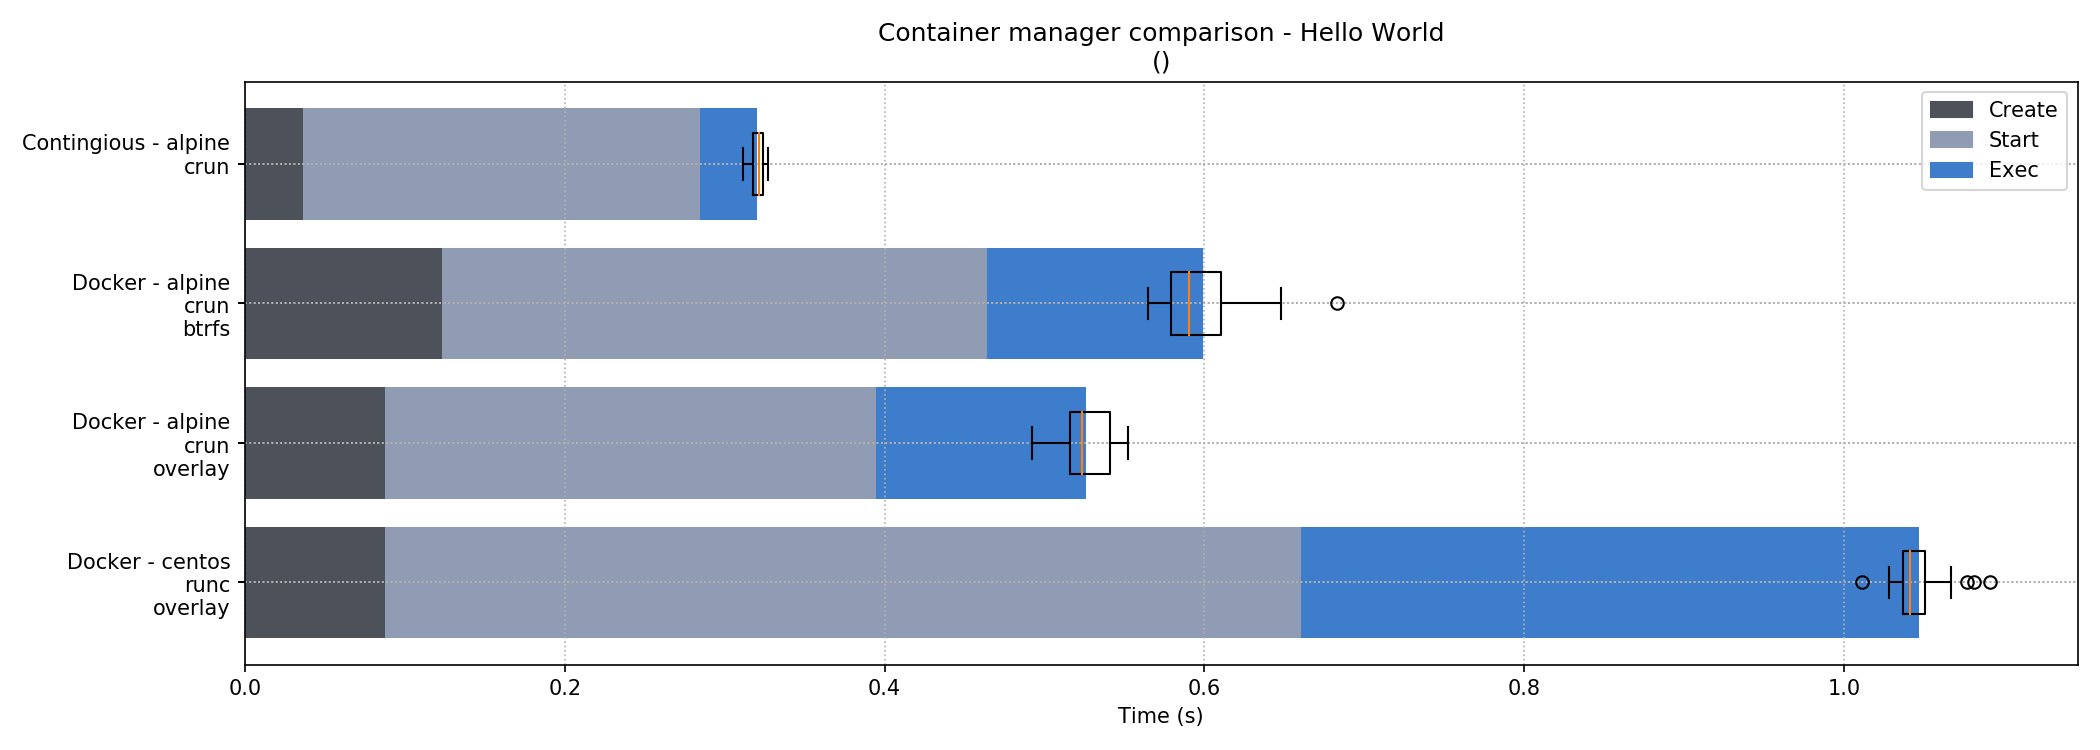
\includegraphics[width=\linewidth]{images/question-2-hello-world.png}
    \caption{Ideal INGInious container manager solution compared to the current configuration of the platform and to the recommended new solution, Hello World test}
    \label{fig:q2:hello-world}
  \end{center}
\end{figure}

In Figure \ref{fig:q2:hello-world} we can see that the gain in performance is real, and we did not give up any of the key requirements of INGInious.  We have the same level of isolation that Docker provides as we rely on crun, we even made it one step further as this solution is completely rootless.

\begin{figure}[h!]
  \begin{center}
    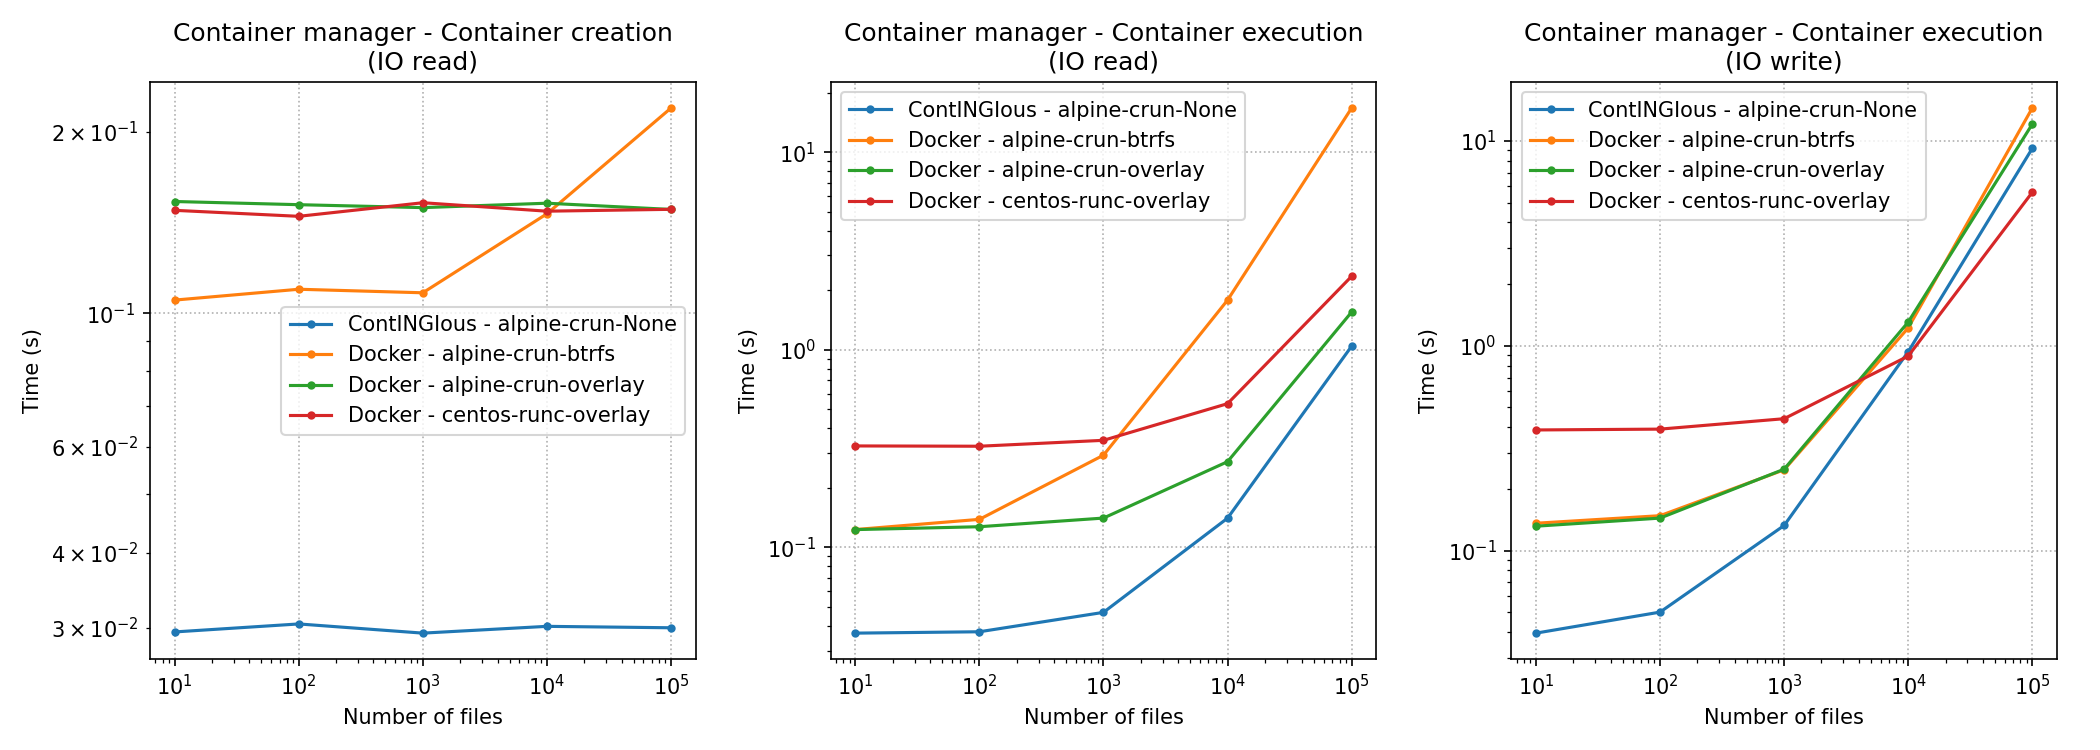
\includegraphics[width=\linewidth]{images/question-2-io.png}
    \caption{Ideal INGInious container manager solution compared to the current configuration of the platform and to the recommended new solution, IO tests}
    \label{fig:q2:io}
  \end{center}
\end{figure}

In Figure \ref{fig:q2:io} we can see that the only battle we lose is with the current INGInious solutions for the writing test, as its \texttt{tar} implementation is more efficient.  Otherwise, reading file is way faster when you do not need to manage different layers of your file system as with overlay, and writing is faster too as, again, we do not need to care about different layers.

\begin{figure}[h!]
  \begin{center}
    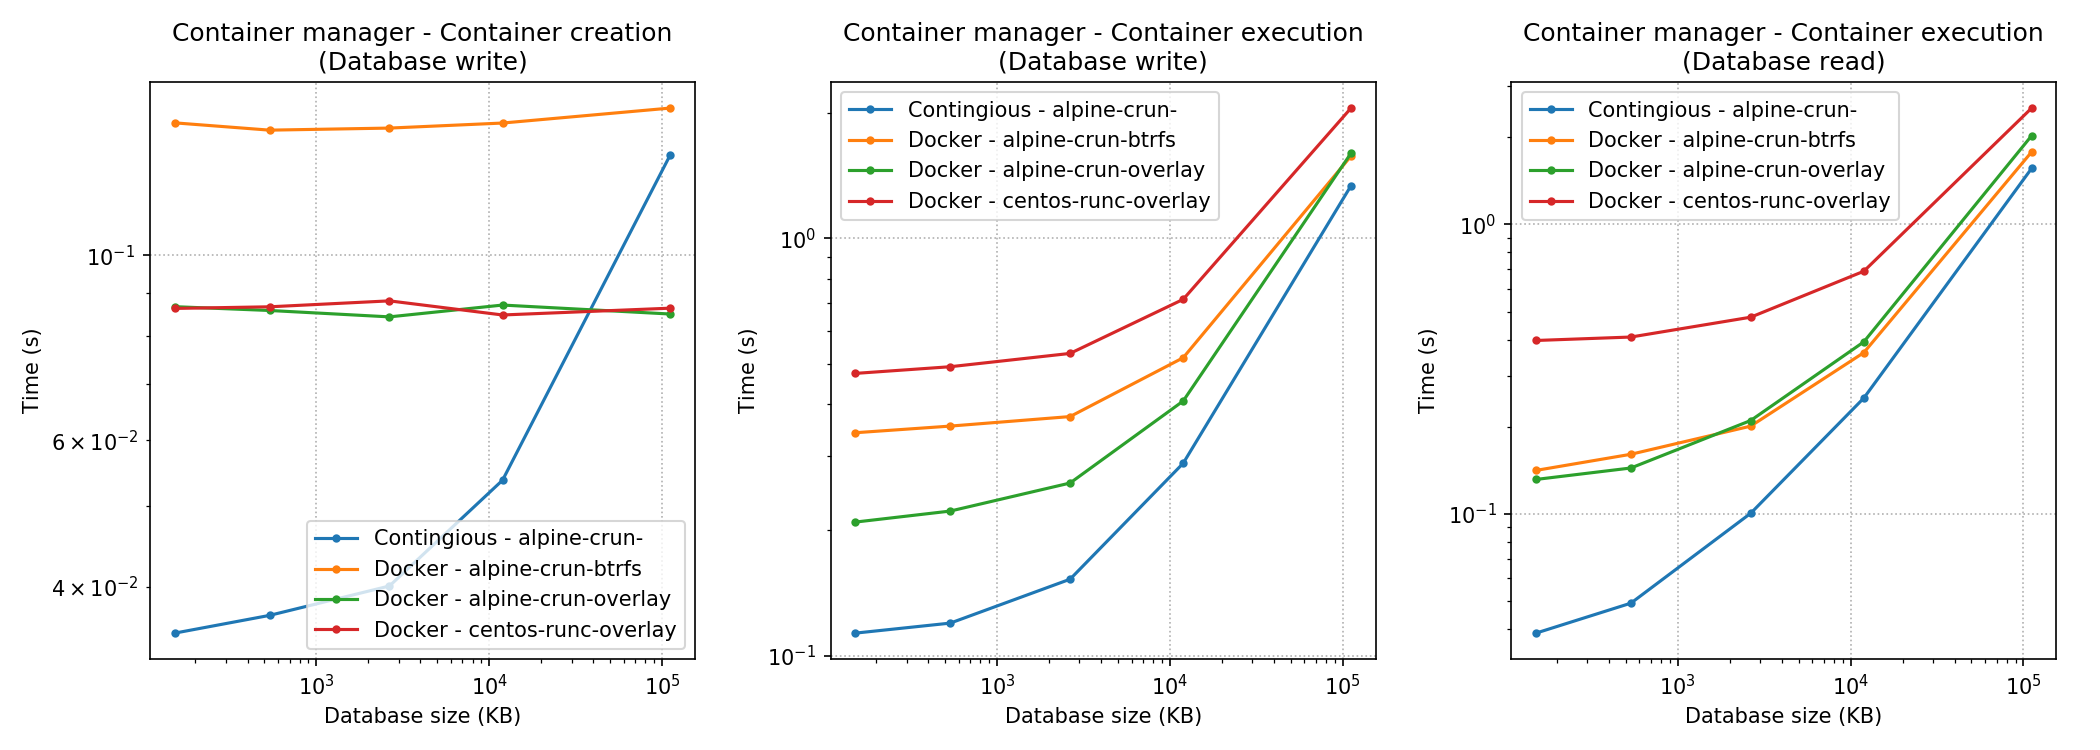
\includegraphics[width=\linewidth]{images/question-2-db.png}
    \caption{Ideal INGInious container manager solution compared to the current configuration of the platform and to the recommended new solution, Database tests}
    \label{fig:q2:db}
  \end{center}
\end{figure}

In Figure \ref{fig:q2:db} we see that this solution is not magical though, copying files before editing them is still costly.  But doing this when creating the container still provides overall better performances than copying the file to a higher layer, as overlay would, just before writing it.  The only alternatives that could beat us for more extreme situations are block-based copy-on-write solutions, as they will not copy the whole file.  That being said, we could probably improve this solution by making use of that feature too, relying on an underlying filesystem that has such capabilities.

\paragraph{}This prototype shows the improvements expected, but there is still work to do before integrating it into INGInious.
\begin{itemize}
  \item Determine for each container which should be the writable part of the file system.  And eventually, optimize those images by centralizing all the writable content.
  \item Create a new image management system.  We do not need to go from scratch though, Buildah\footnote{Buildah is a tool that allows us to easily build and manage OCI images. \href{https://github.com/containers/buildah}{https://github.com/containers/buildah}} could be used, and would even allow us to continue using Docker Hub to store images.
  \item Integrate all the management of the steps of creation and execution of containers in one reliable tool.  For that we do not need to start from scratch, it might be worth taking a look at conmon\footnote{Conmon is the container runtime monitor on which Podman relies.  \href{https://github.com/containers/conmon}{https://github.com/containers/conmon}}.
\end{itemize}

Whether the performance improvement of this solution is worth the effort it would require to put it in place is not my call to make. I like that idea, and I think it would make a great project, but it would also cost some time to set up and maintain.

\section{INGInious opportunities}
We will here consider the last question:
\begin{center}
  \say{\textit{What would be the cost of providing stronger/safer isolation to the containers used by INGInious?  Which opportunities could it bring?}}
\end{center}

By saying "\textit{providing a stronger-safer isolation}" what I mean is more mitigating the risk we take when we let a student execute code in a container, on the host where the platform is running.  The most unsafe solution (still making use of containers) is to run the container as root, with the root user of the container in the hand of the student and mapped to the root of the host.  In theory, this does not do any harm but given past vulnerabilities that have been found in runc, it can happen.  To mitigate this, INGInious currently creates a new user in the container, which has no root privileged (neither inside the container nor outside of it), for the student code to execute.  This limits the range of possibilities of tasks to evaluate with INGInious.  We cannot for example simulate a cluster of machines where the student has root access to deal with any network assignment.

\subsubsection{Rootless containers}
\paragraph{}The first possibility to improve this situation is to go with rootless containers.  We have two alternatives for this: Podman's rootless containers and LXD unprivileged containers.  Docker is also working on a solution but has only limited support for now.  With rootless containers, not only the root inside the container is not root on the host, but also the container runtime is not running as root, which limits a lot the damage that can be done to the infrastructure if a vulnerability in the container runtime is found and exploited.  It also mitigates potential attacks the other way around, for a user on the host that would try to gain root access through a vulnerability of the container manager.  This is only valid for Podman though, as LXD's daemon is running as root, even for unprivileged containers.  Podman could then be installed on the student's machine in computer rooms without too much concern.

\begin{figure}[h!]
  \begin{center}
    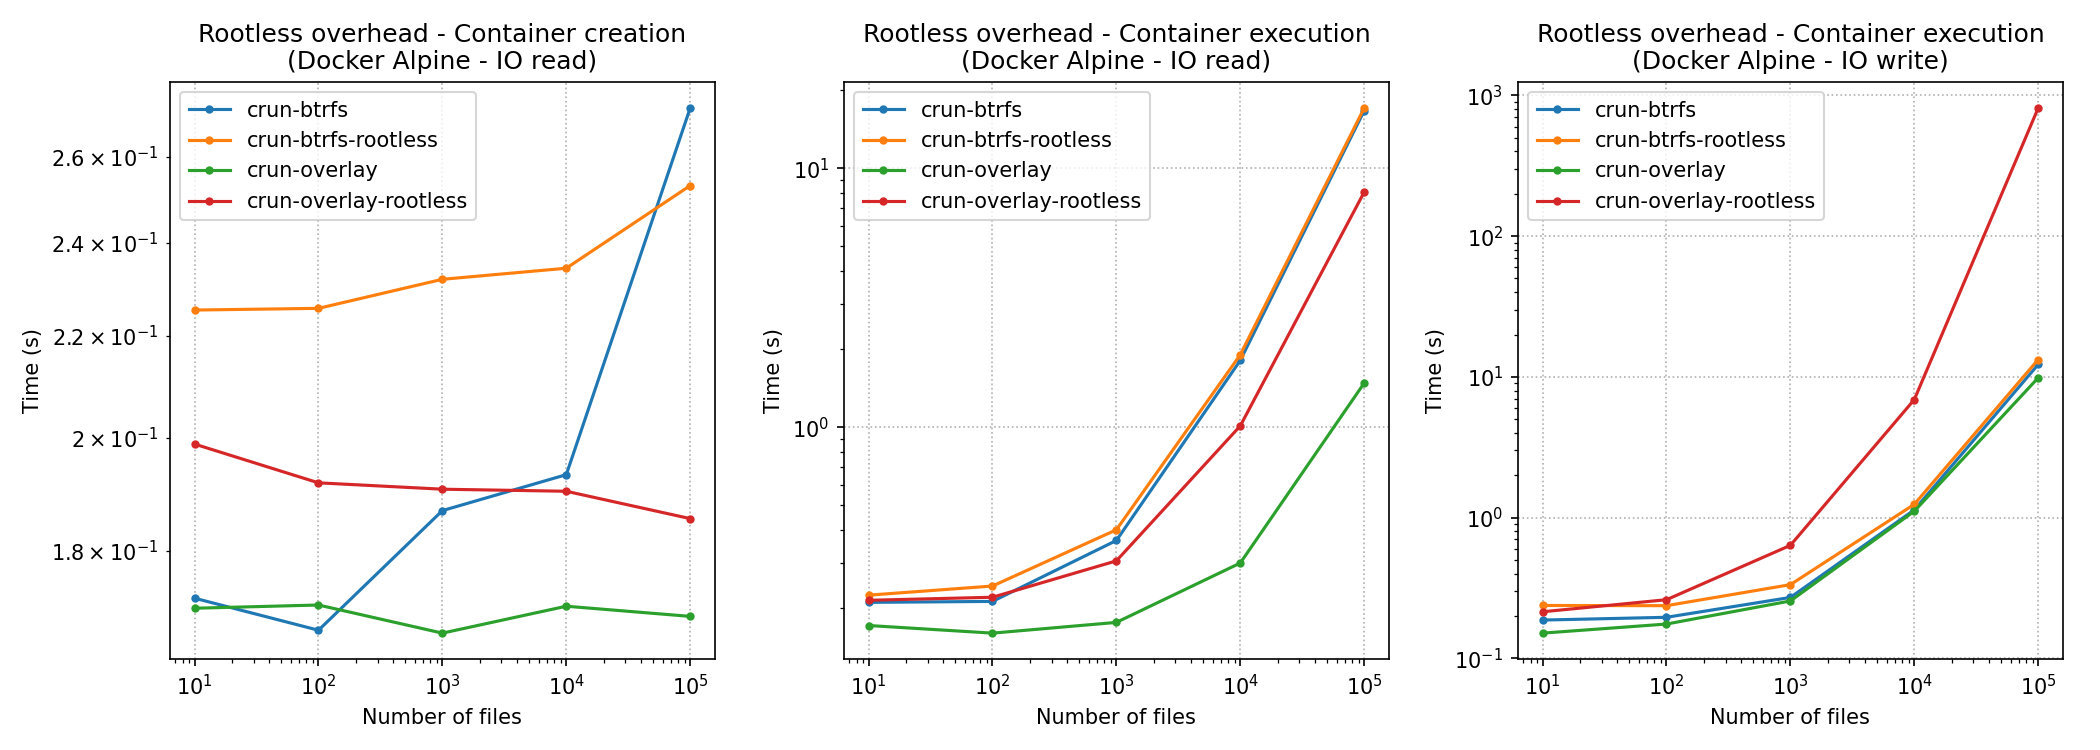
\includegraphics[width=\linewidth]{images/question-3-rootless-io.png}
    \caption{Overhead of rootless containers compared to rootfull ones, IO tests}
    \label{fig:q3:rootless:io}
  \end{center}
\end{figure}

Unfortunately, having rootless containers also comes with a cost as we can see in Figure \ref{fig:q3:rootless:io}.
\begin{itemize}
  \item There is a cost to create, start and execute command into rootless containers with Podman compared to going rootfull with the same container manager.  This is very likely caused by the extra steps required to launch a rootless container with all the functionalities of a rootfull one.  Podman needs first to unshare user and mount namespaces, to be able to make bind mounts on the container filesystem.  It also requires adding a cgroup scope to all the commands that set up the containers, to be sure that the container runtime will later be able to move process created to the cgroup attached to the container.
  \item Because of the lack of \textit{real} root permissions on the machine, rootless containers can not use OverlayFS, instead they use a FUSE\footnote{FUSE, or filesystem in user space, allows for a non-privileged user to create a filesystem in user space instead of kernel space.} implementation of the latest, which, as we can see on the right-most graph, induces great performances loss.  It gets even worse when doing write operations.
  \item One limitation of a rootless container is also the options available for managing the storage of containers (storage drivers), for example, devicemapper is not available.
\end{itemize}

\subsubsection{Virtualization}
\paragraph{}Another solution is to simply strengthen the isolation that protects the host from the student.  And the best solution to do this is to make use of virtualization.  Kata Containers is a great deal for us, it allows us to keep the infrastructure of the platform, only changing the runtime used by Docker, and everything can still be used as before.  Once again, this stronger isolation level could open the gate to new assignments that would require the student to have root access in the container.

\paragraph{}However, as we already saw earlier when comparing runtimes, virtualization adds a cost, mainly to container start-up, but also on creation and execution.

In Figure \ref{fig:q3:virtualization:io}, we can notice that unlike for crun, the overlay storage driver behaves way worse than devicemapper.  This is also the case for all other storage drivers. It seems that runtime solutions with virtualization take much more advantage of devicemapper than other drivers.  And passed a certain point, Kata Containers using Qemu even perform better than crun, both in read (compared to crun with devicemapper) and write (compared to crun with overlay or devicemapper).

\begin{figure}[h!]
  \begin{center}
    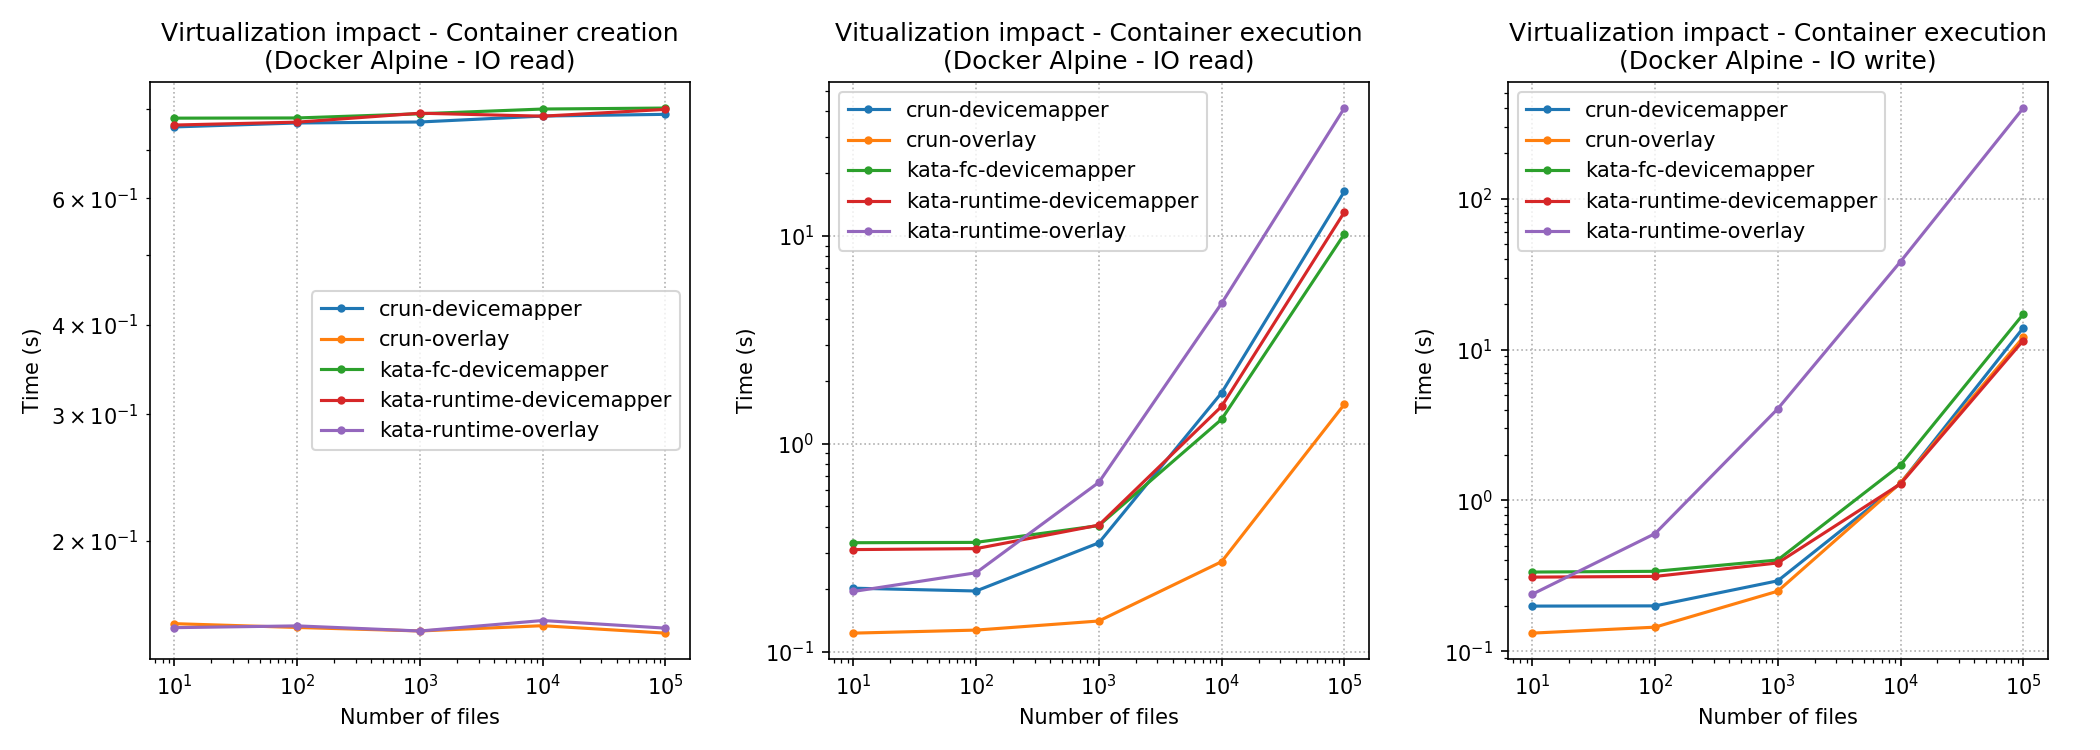
\includegraphics[width=\linewidth]{images/question-3-virtualization-io.png}
    \caption{Cost of virtualization on container creation and execution, IO tests}
    \label{fig:q3:virtualization:io}
  \end{center}
\end{figure}

We can make the same observation in Figure \ref{fig:q3:virtualization:db} with the exception than, for some reason, Kata Containers using Firecracker seems to handle read operations on big files much better than when using Qemu.

\begin{figure}[h!]
  \begin{center}
    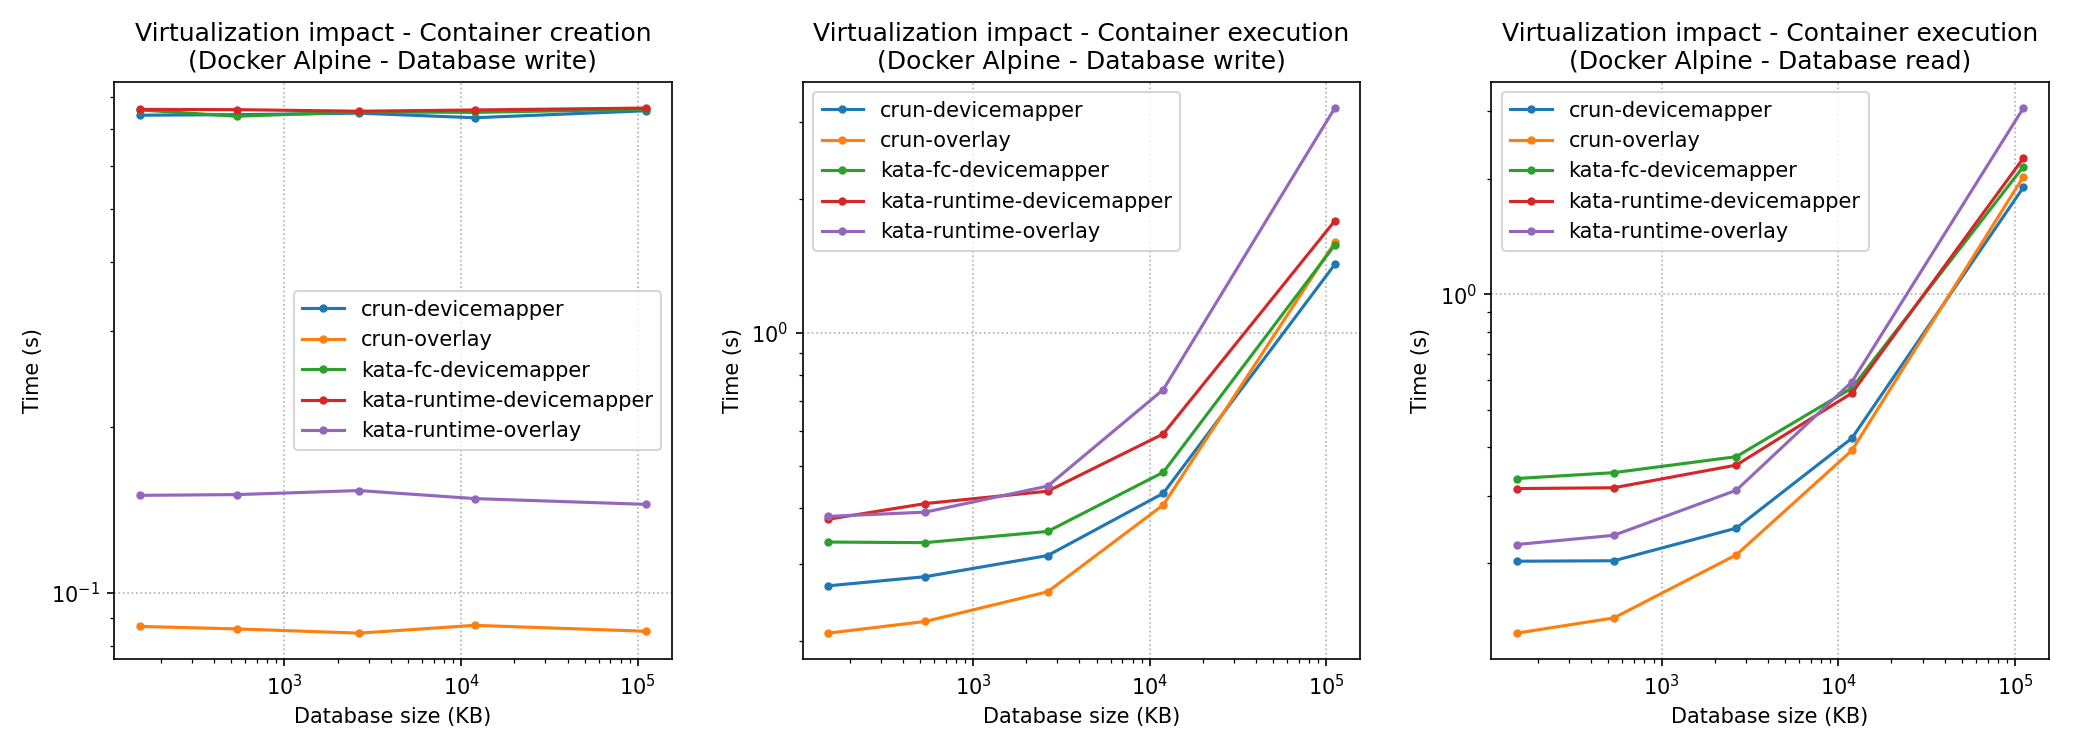
\includegraphics[width=\linewidth]{images/question-3-virtualization-db.png}
    \caption{Cost of virtualization on container creation and execution, IO tests}
    \label{fig:q3:virtualization:db}
  \end{center}
\end{figure}

One more great thing about Kata Containers is that every container in the same pod (a group of containers, linked together, that serves a common global purpose) will be grouped inside the same VM (still in separate containers), this will reduce the overhead by container caused by virtualization as the size of the pod grows.  This could be convenient for assignments where multiple containers need to be managed by a single student.  Unfortunately, to make use of this feature, the container manager needs to have some kind of pod mechanism, which is not the case of Docker.  Podman, Kubernetes or others can do that.
